% Author: Ernesto Diaz
% Panther ID: 4890534
There are three important characteristics of frequency distributions to comprehend
that are consistent regardless of the visualization used.

\subsection{Measures of Central Location}

Oftentimes when a frequency distribution is graphed it is common for a significant
amount of data points to cluster around a central value. This clustering is referred to
as the central location or central tendency of a frequency distribution. Once the 
value that a distribution centers around is known, it can be used to further 
characterize the rest of the data in the distribution. To calculate a central value 
several methods exist with each method producing somewhat of a different result. 
Collectively these methods can be referred to as ``Measures of Central Location`` 
and the three most commonly used are:

\begin{enumerate}
    \item Mean: the sum of all values divided by the total number of values.
    \item Median: the middle number in an ordered data set.
    \item Mode: the most frequent value.
\end{enumerate}

These three measures are best used in combination with one another. This is because 
they have complementary strengths and weaknesses. The mode can be used for any 
level of measurement, but it is most meaningful for nominal and ordinal values.
The median can only be used on data that exhibits some type of order and the mean 
can only be used on interval and ratio values of measurement. This because it requires 
equal spacing between adjacent values or scores in the scale \cite{c12}. Most of 
the time depending on the dataset, only one or two of these measures are applicable 
at any given time.

\subsection{Measures of Dispersion}

A second property of frequency distributions is dispersion also know as variation, which 
is defined as the spread of a distribution out from its central value. The dispersion 
of a frequency distribution is independent of its central location. Figure \ref{figure:central_location} 
illustrates this fact, by showing the graph of three theoretical frequency distributions that have 
the same central location but different amounts of dispersion. Some of the more common
measures of dispersion that are used include the following:

\begin{enumerate}
    \item Range: the difference between the largest and the smallest observation 
    in the dataset.
    \item Interquartile Range (IQR): the difference between the 25\textsuperscript{th} and 
    75\textsuperscript{th} percentile (also called the first and third quartile).
    \item Standard Deviation: Measures the spread of data about the mean. 
\end{enumerate}

Much like measures of central location, measures of dispersion have their own set of
strengths and weaknesses. For instance, the biggest advantage of the range is that 
it is very easy to calculate. But the main disadvantage to be aware of is its 
sensitivity to outliers. Moreover, the range does not take into account all 
the observations in a data set. Likewise, in some situations it might be more informative 
to actually provide the minimum and maximum values rather than the range a singular value \cite{c1}.

The interquartile range has a rather interesting advantage given that it is not 
affected by extreme values. Due to this the interquartile range can be used as 
a measure of variability if extreme outliers do exist in the dataset. However, its 
main disadvantage is that it is not amenable to mathematical manipulation.

Standard Deviation (SD) is perhaps the most famous and widely used measure in dispersion
calculations. The reason why is because if the observations are from a normal distribution, 
then we can assume that 68\% of observations lie between the mean and $\pm1$ SD, 95\% of 
observations lie between the mean and $\pm{2}$ SD and 99.7\% of observations lie between 
the mean and $\pm{3}$ SD \cite{c1}. The other advantage of standard deviation is that along with the 
mean it can be used to detect skewness. However, its biggest disadvantage is its 
inability to be used as an appropriate measure of dispersion for data this is 
already skewed.

\begin{figure}
    \centering
        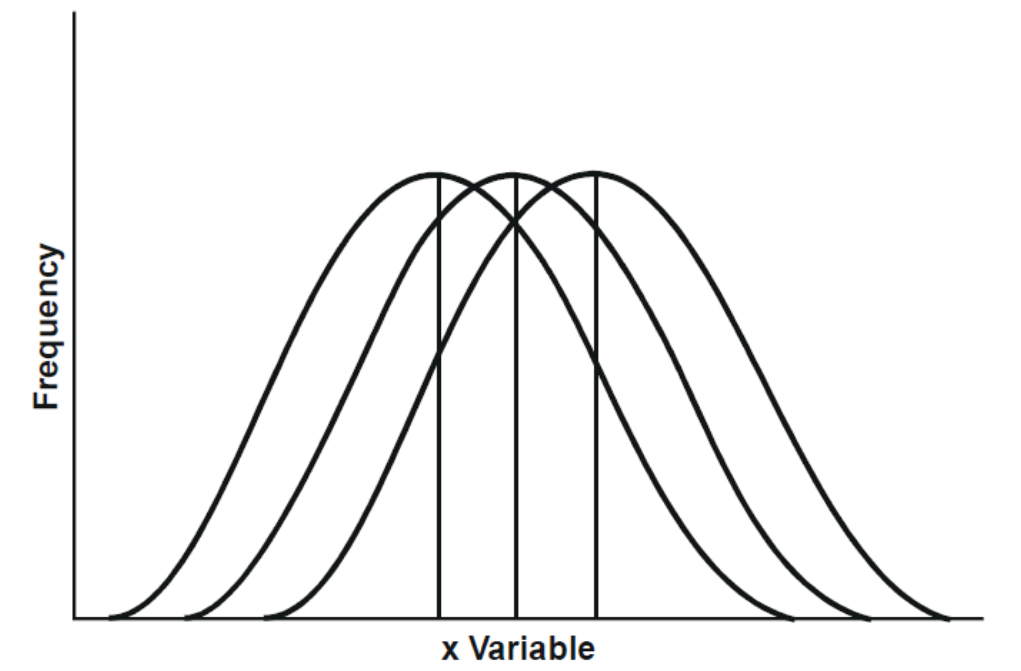
\includegraphics[height=4cm]{figures/diff_central_location.png}
    \caption{Three curves identical in shape with different central locations \cite{c13}.}
    \label{figure:central_location}
\end{figure} 

\subsection{Skewness}

Skewness is a measure of symmetry, or more precisely, the lack of symmetry. A 
distribution is symmetric if it looks the same to the left and right of the center 
point. The skewness for a normal distribution is zero, and any symmetric data 
should typically have a skewness near zero. Negative values for the skewness 
indicate that a dataset has a majority of its data points skewed left while positive 
values indicate a majority of data points are skewed right. For context when we
say "skewed left", we mean that the left tail is long relative to the right tail. 
Similarly, "skewed right" means that the right tail is long relative to the 
left \cite{c13}. Luckily, we can define the skewness of a distribution with the 
following formula:
\begin{equation}
    Skewness = \sum{}{} \frac{(X_i-\bar{X})^3}{ns^3}
\end{equation}
where $n$ is the sample size, $X_i$ is the $i\textsuperscript{th}$ $X$ value, $\bar{X}$ 
is the average and $s$ is the sample standard deviation \cite{c14}. However, most software 
tools such as Microsoft Excel take into account the sample size as well. Therefore,
we can slightly modify the formula to the following:
\begin{equation}
    \begin{split}
        Skewness & = \frac{n}{(n-1)(n-2)}\sum{}{} \frac{(X_i-\bar{X})^3}{s^3} \\
        & = \frac{n}{s^3(n-1)(n-2)}(S_{above} - S_{below})
    \end{split}
\end{equation}
In practice, as the sample size increases the difference in the results that these 
two formulas potentially produce is relatively small so either one can be used with 
confidence. 
